\chapter{Background}
\label{chp:background}

In this chapter we'll discuss some technical aspects of video conferencing that affects how we reason about the problem, and evaluate what sort of trade-offs established actors on the market have made.

\section{WebRTC}

This thesis is largely inspired by the efforts of the \gls{w3c} in standardizing \gls{webrtc}, a technology which enables direct browser-to-browser communication. Building on \gls{webrtc}, services like Telenor Digital's appear.in and Telefonica's Hello have come to life, ushering in a new age of communication that does not depend on the traditional GSM infrastructure, but is fueled by faster Internet connections and more capable smartphones.

It's interesting to note that many of the largest WebRTC communication platforms (like appear.in and Hello, as mentioned) we've seen so far have been developed by the largest players in the traditional communication field, and not from any independent outsider. The big telephone companies do have capabilities other actors don't enjoy, such as being able to freely route calls back over GSM as a fallback solution in case a person is not reachable online, but this has not been a selling point for the services so far. The services have also largely been focused on video conferencing, even though the technology is equally well-suited for pure voice conversations or text-based communication.

In any case, the hard part of the problem is video conferencing, as the demands on the user equipment and connection is far greater than what will ever be exercised by voice or text. Group conversations on appear.in is today artificially limited to 8 people, but often the parties in the conversation will experience practical limits below this due to insufficient bandwidth or CPUs not capable of encoding enough parallel video streams.

The dynamic routing scheme proposed in this thesis is largely independent of underlying technology, but is intended to be built on top of \gls{webrtc}. The requirements to implement the suggested solution is that the platform allows clients to establish connections with a given starting bitrate (which WebRTC allows through modifying the SDP offer), and that streams can be routed arbitrarily. As connections have to be established in an ad-hoc way out-of-band in WebRTC, as long as the parties involved all share session keys, this should also be feasible.

There are practically three different implementations of the WebRTC specification today; \texttt{libjingle}, which powers Chrome and Opera; Mozilla's, which is tightly coupled with Firefox; and OpenWebRTC, a mobile-first framework for native apps, started by Ericsson Research. There's also WebRTC Microstack\footnote{\url{http://opentools.homeip.net/webrtc}}, but they are data-channel only, which means they don't support the audio/video APIs. There's also been some interest in a pure JavaScript implementation to ease development of WebRTC-aware server-side applications\footnote{\url{https://github.com/webrtcftw/goals/issues/1}}, but that project doesn't seem to have had much activity since late 2014.


\section{A Technical Look at Video Conferencing}

\subsection{Encoding}

The naïve approach to encoding video is to encode the raw stream from the web camera into several client-optimized streams for transmission. However, H.264 can be encoded in a \gls{svc} manner, which layers several different streams with different bandwidths into a single stream. A node receiving a \gls{svc} stream can extract layers with the bitrate desired, without re-encoding the entire stream. With VP8 this is sadly not possible, and the only alternative is to utilize a \gls{sfu}, a technique where several streams are sent to the same endpoint, which can then select which of the streams to forward to the different endpoints. This is not as efficient as sending only a single stream however, and the encoding step is costlier in terms of CPU-time.

Google has entered a collaboration with Vidyo \cite{vp9-vidyo} to bring \gls{svc} to VP9, which might bring free-to-use \gls{svc} to WebRTC. While both Firefox and Google support decoding VP9 today \cite{vp9-support}, encoding is not yet an option for either.

One of the big issues regarding video codecs is the ongoing war between H.26x and VPx, which boils down to licensing issues. VPx is royalty-free for anyone to use and implement, and has thus gained lots of support in the free software community. H.26x is protected by patents, and products shipped with H.26x support needs to aquire a license, which motivated the browsers to start pursuing a free\footnote{As in speech} option which became the WebM project that develops VPx.

Both H.26x and VPx can be hardware-accelerated, and is deployed in several products on the market. Most deployed solutions are decode only, but some, like the Nvidia Tegra 4, also supports encoding \cite{nvidia-hw-encode}. The WebM project maintains open designs for hardware encoders and decoders for VPx.


\subsection{Continuous Presence vs. VAS}

There are mainly two different ways to do video conferencing, Continuous presence and \acrfull{vas}. Continuous presence means that all parties in the conversation is visible to all other parties at the same time. \gls{vas} means that only one party is visible, typically the one detected by the system as talking at any given time. There's also hybrid schemes, sort of how Google Hangouts does it, where there's a VAS, but the user can override locally who should be shown up big.

Clearly, in larger conversations, there's a huge difference in network impact of the two technologies, as a VAS-based solution will always just require a single video link in and out, while continuous presence will scale bandwidth requirements linearly with the size of the conversation. \autoref{fig:service-possibilities} summarizes the possible services that can be provided for different amounts of available bandwidth. A minimal video unit is the smallest bitrate it makes sense to encode video in. This will be service dependent, but we can imagine $\approx$500kbps to be reasonable.

\begin{figure}
    \centering
    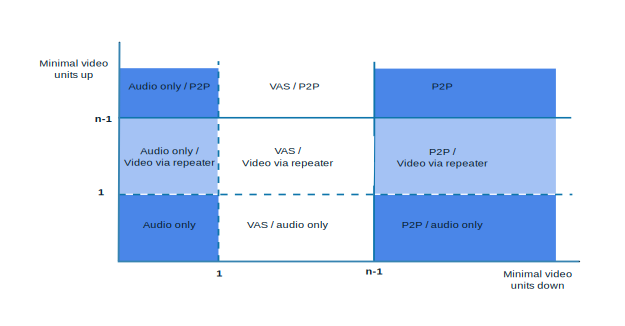
\includegraphics[width=\textwidth]{commcap}
    \caption{The possible services for different upload/download bandwidths. A minimal video is the smallest bitrate where it makes sense to send video. Dark blue is what appear.in can provide today (audio only requires manual configuration), light blue is what's possible with the solution suggested later in this thesis.}
    \label{fig:service-possibilities}
\end{figure}

Continuous presence can be accomplished both in a peer-to-peer topology and centralized topologies, but since a \gls{vas} requires insight into the video streams (or at least, the audio streams) to select who is forwarded at any given time, they are only realizable if all the video streams go through centralized servers. In theory it's possible to expand the system to work over peer-to-peer as well, by having each peer use a low-bandwidth data channel to tell nodes whether it's currently speaking or not, but this requires that video streams can be quickly started, stopped, and that the system gracefully handles collisions without falling over. The problem is non-trivial, as it's essentially a question of distributed consensus. Having a single place that handles the question of who's active is a lot simpler to reason about and implement.

Note that even though video is switched in a \gls{vas}-system, everyone's audio is usually sent to everyone.

\subsection{NAT and Firewalls}

The presence of \gls{nat} makes connection estalishment between users harder than necessary, as nodes behind a NAT are not aware of their external IP address and port. The \gls{ice} framework providers two protocols that can be implemented to alleviate parts of the problem; \gls{stun} and \gls{turn}. STUN is a very lightweight protocol used to discover your externally visible network address, while TURN-servers can act as intermediaries between users that cannot reach each other directly due to firewalls. TURN servers are often the biggest server expense for WebRTC-based solutions, since the provider have to take the cost for the bandwidth consumed by the users.

For WebRTC, STUN would be needed even in the absense of NATs, since JavaScript does not have any APIs for binding to ports, only for establishing outgoing connections. Thus there's no way for a node to announce the port it's accepting connections to before it has established a connection outward, a chicken-and-egg problem STUN resolves.


\section{The current providers}

A selection of widely-known video conferencing solutions today, with significantly different network architectures are summarized in the following table.

\begin{center}
	\label{tab:existing-solutions}
	\begin{tabular}{| l | l |}
		\hline
		\textbf{Service} & \textbf{Description} \\ \hline
		appear.in & Browser-based peer-to-peer WebRTC service \\ \hline
		Google Hangouts & Browser-based with Vidyo-powered \gls{sfu} \\ \hline
		Microsoft Skype & Downloadable app, proprietary protocol \\ \hline
		Cisco TelePresence & Custom hardware, self-hosted or cloud service \\ \hline
	\end{tabular}
\end{center}

Notably absent here is FaceTime, Apple's video conversation service bundled with their devices. FaceTime's absence in this thesis is due to the lack of support for more than two people in a conversation (thus being more video \emph{chat} than video \emph{conference}), and the lack of support for non-Apple devices.

We also note that Mozilla just entered the market in collaboration with Telefonica with their Hello service, bundled with recent versions of Firefox\footnote{https://www.mozilla.org/en-US/firefox/hello/}. Hello essentially provides the same service as appear.in, just bundled with the browser. Thus anything we say about appear.in applies to Firefox Hello as well (and all other peer-to-peer WebRTC services), and we'll therefore not consider them separately.

Let's take a more detailed look at these services.

\subsection{appear.in}

appear.in is a free peer-to-peer service built on WebRTC that does not require sign-ups or installation of add-ons to your browser. Due to the WebRTC requirement the service is available to anyone using a recent version of either Google Chrome, Mozilla Firefox or Opera, while the OS-provided browsers (Internet Explorer and Safari) have notably not implemented WebRTC yet.\footnote{Browser support for WebRTC can be tracked at \url{http://iswebrtcreadyyet.com/}}

appear.in is the only solution studied in this thesis that allow anonymous communication. The combination of continuous presence and a peer-to-peer topology makes the device and network requirements scale linearly with the number of people in a conversation. The service is limited to maximum 8 people in a conversation.


\subsection{Google Hangouts}

Google Hangouts is alongside appear.in the only other service covered in this thesis based in the browser. Hangouts is a merge of several earlier Google communication solutions like Google Talk, Google+ Messenger and the Hangouts feature from Google+. The service uses a Vidyo-provided \gls{sfu}, and VP8/9 over WebRTC in a non-standard configuration on Chrome \cite{hangouts-webrtc}, and requires a plugin on other browsers \cite{google-hangouts-support}. A conversation is limited to 10 people.

Hangouts requires you to setup a public Google+ profile, which makes the barrier of entry higher than for most of the other services tested in this thesis. Hangouts is free to use, but room capacity can be increased to 15 people in the paid Google Apps for Work version.


\subsection{Skype}

Skype is probably the most well-known of the solutions we're looking at, being among the first to offer free video conferencing for personal use way back in 2003. Skype was also among the first to provide a VoIP solution inter-operating with \gls{pstn}, easing the barrier of entry for new users. The original Skype topology was peer-to-peer, built on top of the file-sharing protocol powering Kazaa, which was developed by the same founders \cite{skype-history}.  The Skype protocol is proprietary and requires installing the Skype application. For NAT-traversal, Skype initially used other Skype users known as supernodes as intermediaries, performing the same role as TURN-servers in the ICE framework. After the Microsoft acquisition in 2011, Skype dropped the client-hosted supernodes in favor of Microsoft-hosted ones, justified as a means to improve performance and security for users \cite{skype-topo-change}. A Skype conversation has a soft limit on five people for the best user experience, and a hard limit on 10 users.

Skype requires a standalone application to run, which is available on pretty much every platform out there, including Windows, Mac, Linux, Android, iOS, Windows Phone, BlackBerry, most tablets, TVs, gaming consoles and more. The benefit is close access to hardware and GPUs for more efficient video encoding, the downside is the lack of open protocols, standardization and transparency.


\subsection{Cisco}

Cisco offers both on-premises, off-premises and hybrid solutions for video conferencing, aimed at the enterprise market. Video is routed through either self-hosted or cloud \glspl{mcu} or \glspl{sfu}, using \gls{sip} and H.323 for call establishment \cite{cisco-arch}. In the case of only two people in a conversation, calls can be established peer-to-peer. H.323 allows interoperability with devices on legacy networks like the \gls{pstn}, such as ISDN videophones, through H.320 gateways. Their core offering is specialized hardware and dedicated rooms for video conferencing (so called immersive video conferences), but they also have a free service that can be run on end-user computers.
